\subsection*{Problema 20}

\noindent\textbf{Enunciado:}
Calcular la integral indefinida:
\begin{equation*}
\int \dfrac{x + 2}{(x - 1)\sqrt{x^2 + 1}} \, dx
\end{equation*}

\noindent\textbf{Solución:}
Para simplificar el integrando, aplicamos la sustitución lineal $u = x - 1$, de donde se deduce que $x = u + 1$ y el diferencial es $dx = du$.

Sustituyendo estas expresiones en la integral original, obtenemos:
\begin{align*}
\int &\dfrac{(u + 1) + 2}{u \sqrt{(u + 1)^2 + 1}} \, du \\
&= \int \dfrac{u + 3}{u \sqrt{u^2 + 2u + 2}} \, du
\end{align*}

Separamos la integral en dos partes para facilitar su integración:
\begin{align*}
= &\int \dfrac{u}{u \sqrt{u^2 + 2u + 2}} \, du \\
&+ \int \dfrac{3}{u \sqrt{u^2 + 2u + 2}} \, du
\end{align*}

Simplificando la primera integral y reestructurando la segunda:
\begin{align*}
= &\int \dfrac{du}{\sqrt{u^2 + 2u + 2}} \\
&+ 3 \int \dfrac{du}{u \sqrt{u^2 + 2u + 2}}
\end{align*}

Completamos el binomio en el radical: $u^2 + 2u + 2 = (u + 1)^2 + 1$. Para la segunda integral, aplicamos la sustitución inversa $z = \dfrac{1}{u}$, con lo cual $dz = -\dfrac{1}{u^2}du$ y $u = \dfrac{1}{z}$:
\begin{align*}
= &\int \dfrac{du}{\sqrt{(u + 1)^2 + 1}} \\
&- 3 \int \dfrac{dz}{\sqrt{1 + 2z + 2z^2}}
\end{align*}

Resolviendo ambas integrales mediante fórmulas estándar de integración:
\begin{align*}
= &\ln\left| (u + 1) + \sqrt{u^2 + 2u + 2} \right| \\
&- \dfrac{3}{\sqrt{2}} \ln\left| (2z + 1) + \sqrt{4z^2 + 4z + 2} \right| + C
\end{align*}

Regresando a la variable original $x$ mediante $u = x - 1$ y $z = \dfrac{1}{x - 1}$:
\begin{align*}
F(x) = &\ln\left| x + \sqrt{x^2 + 1} \right| \\
&- \dfrac{3}{\sqrt{2}} \ln\left| \dfrac{x + 1}{x - 1} + \sqrt{\dfrac{x^2 + 1}{(x - 1)^2}} \right| + C
\end{align*}

Esta expresión representa la antiderivada general de la función dada.

\begin{figure}[H]
	\centering
	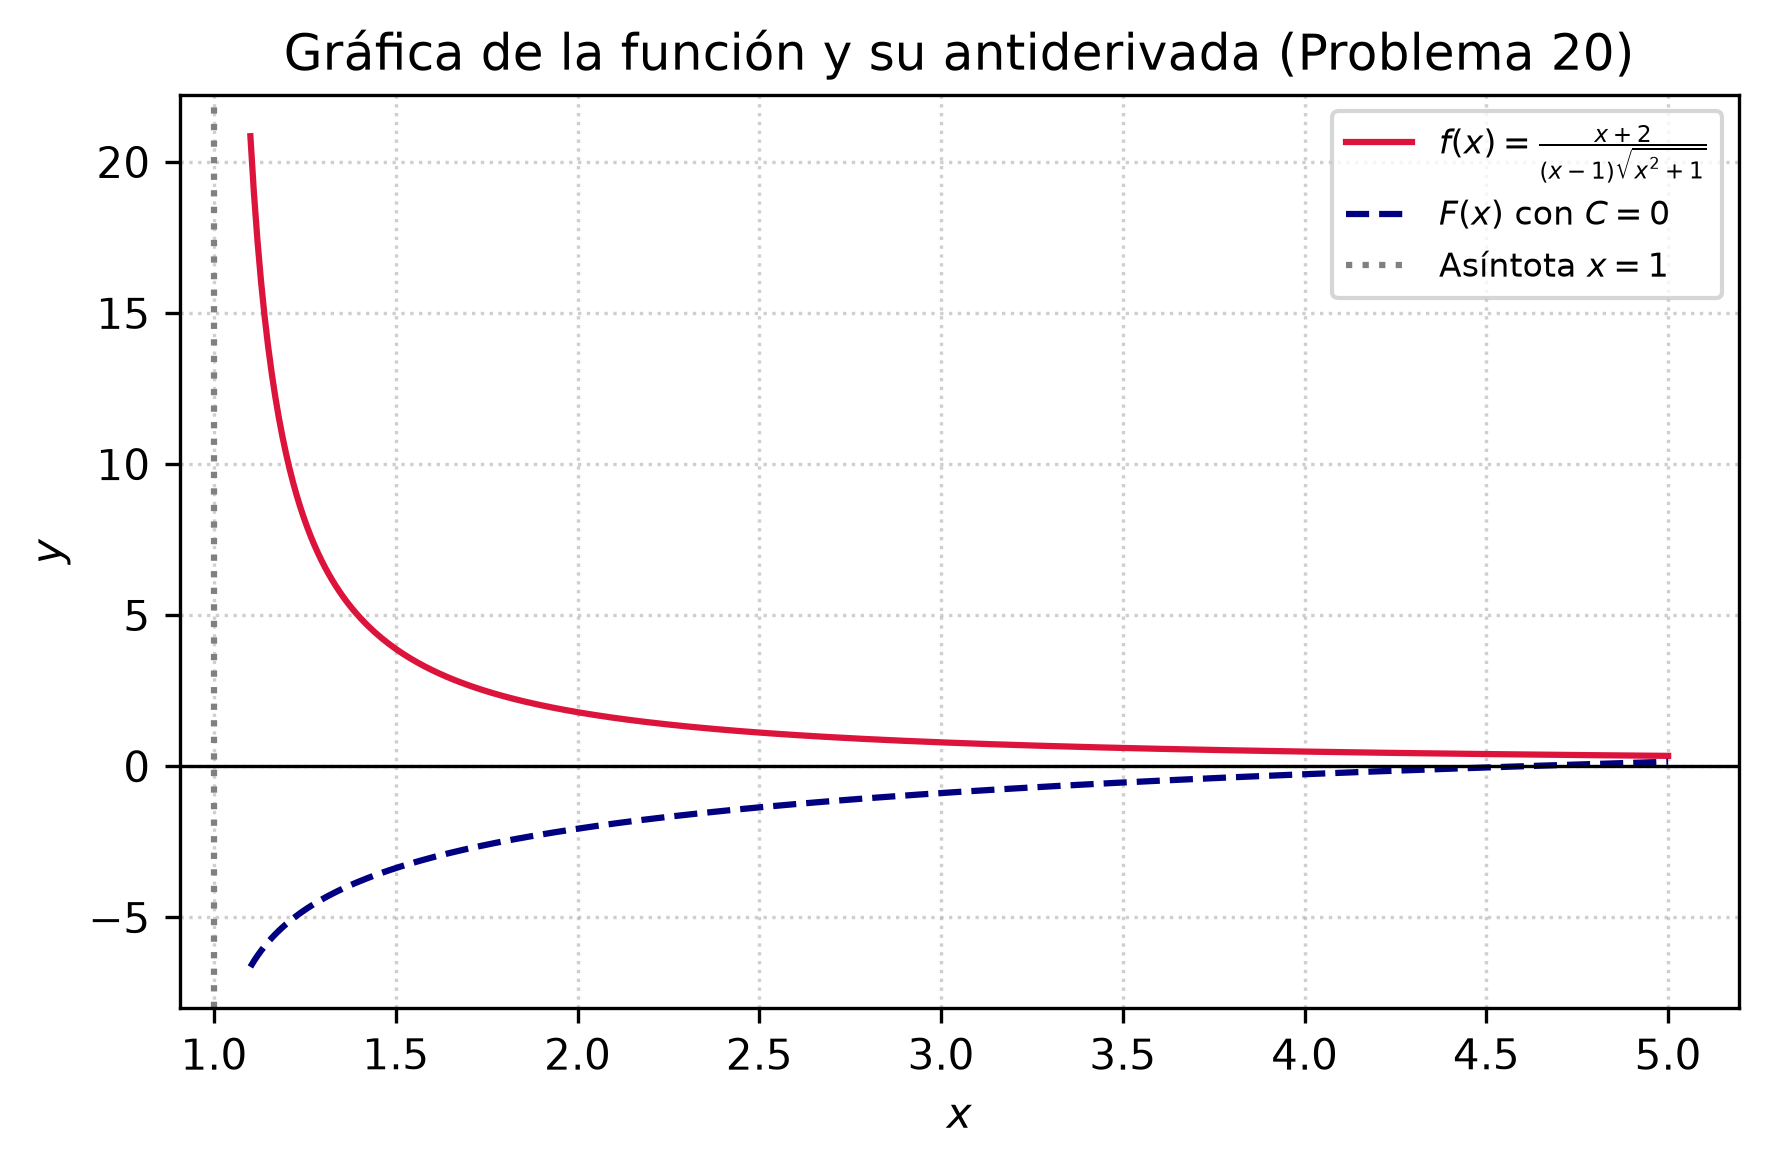
\includegraphics[width=\columnwidth]{semana_05/graficas/SEM05_P20_grafica.png}
	\caption{Representación gráfica de $f(x)$ y su antiderivada $F(x)$ evaluada para la constante de integración $C = 0$ (Problema 20).}
	\label{fig:problema20}
\end{figure}
